\documentclass{vldb}


\usepackage{enumitem}
\usepackage{framed}
%\usepackage[11pt]{moresize}
\usepackage{cprotect}
\usepackage{enumitem}
\usepackage{listings}
\usepackage{amstext}
\usepackage{amstext}
\usepackage{pdfpages}
\usepackage{alltt}
\usepackage{epstopdf}
\usepackage{xspace,colortbl}
\usepackage[USenglish]{babel}
\usepackage{multirow}
\usepackage[hyphens]{url}
\usepackage{subfigure}
\usepackage{graphicx}%%
\usepackage{amssymb}
\usepackage{fmtcount}
\usepackage{amsfonts}
\usepackage{xspace}
\usepackage{amsmath}
\usepackage{multirow}
\usepackage[mathscr]{eucal}
%\usepackage{psfrag}
\usepackage{colortbl}


\usepackage{amsmath,amssymb}
\usepackage[linesnumbered, ruled,vlined]{algorithm2e}

\usepackage{caption}
\usepackage{graphicx}

\usepackage{bm}
\usepackage[nospace]{cite}
\usepackage{csquotes}
\usepackage{enumitem}
\usepackage{times}

%\lstset{basicstyle=\normal\ttfamily,breaklines=true}
%\lstset{framextopmargin=50pt}

\usepackage{cleveref}

\usepackage{balance}

%\linespread{0.99}

\makeatletter
\def\@copyrightspace{\relax}
\makeatother


\DeclareMathOperator*{\argmin}{arg\,min}
\DeclareMathOperator*{\argmax}{arg\,max}
\newcommand*{\QEDB}{\ensuremath{\square}}%



\begin{document}


\newtheorem{theorem}{Theorem}
\newtheorem{example}{Example}
\newtheorem{definition}{Definition}
\newtheorem{problem}{Problem}
\newtheorem{property}{Property}
\newtheorem{proposition}{Proposition}
\newtheorem{lemma}{Lemma}
\newtheorem{corollary}{Corollary}

\newcommand{\detectlib}{\texttt{IsoDetect}\xspace}
\newcommand{\company}{\texttt{Company X}\xspace}
\newcommand{\cond}{\textrm{pred}\xspace}
\newcommand{\dataset}{data set\xspace}
\newcommand{\datasets}{data sets\xspace}
\newcommand{\spview}{\textsf{SPView}\xspace}
\newcommand{\fjview}{\textsf{FJView}\xspace}
\newcommand{\aggview}{\textsf{AggView}\xspace}
\newcommand{\hashfunc}[1]{\textsf{hash}(#1)\xspace}
\newcommand{\hashop}{\textsf{hash}\xspace}
\newcommand{\nsc}{\textsf{NormalizedSC}\xspace}
\newcommand{\rsc}{\textsf{RawSC}\xspace}

\newcommand{\avgfunc}{\ensuremath{\texttt{avg} }\xspace}
\newcommand{\maxfunc}{\ensuremath{\texttt{max} }\xspace}
\newcommand{\minfunc}{\ensuremath{\texttt{min} }\xspace}
\newcommand{\histfunc}{\ensuremath{\texttt{histogram\_numeric} }\xspace}
\newcommand{\countfunc}{\ensuremath{\texttt{count}}\xspace}
\newcommand{\sumfunc}{\ensuremath{\texttt{sum} }\xspace}
\newcommand{\varfunc}{\ensuremath{\texttt{var} }\xspace}
\newcommand{\stdfunc}{\ensuremath{\texttt{std} }\xspace}
\newcommand{\covfunc}{\ensuremath{\texttt{cov} }\xspace}
\newcommand{\corrfunc}{\ensuremath{\texttt{corr} }\xspace}
\newcommand{\medfunc}{\ensuremath{\texttt{median} }\xspace}
\newcommand{\percfunc}{\ensuremath{\texttt{percentile} }\xspace}
\newcommand{\havingfunc}{\ensuremath{\texttt{HAVING} }\xspace}
\newcommand{\selectfunc}{\ensuremath{\texttt{select} }\xspace}
\newcommand{\ratio}{\ensuremath{\rho }\xspace}


\newcommand{\insertion}{\ensuremath{\texttt{INSERT} }\xspace}
\newcommand{\update}{\ensuremath{\texttt{UPDATE} }\xspace}
\newcommand{\delete}{\ensuremath{\texttt{DELETE} }\xspace}

\newcommand{\sysfull}{AlphaClean\xspace}
\newcommand{\sys}{AlphaClean\xspace}
\newcommand{\sysnospace}{AlphaClean}


\newcommand{\tbl}[1]{\textsf{#1}\xspace}
\newcommand{\field}[1]{\textsf{#1}\xspace}
\newcommand{\cost}{\textrm{cost}\xspace}
\newcommand{\ans}{\textsf{ans}\xspace}
\newcommand{\dans}{\Delta\textsf{ans}\xspace}
\newcommand{\cqp}{correction query processing\xspace}
\newcommand{\Cqp}{Correction query processing\xspace}

\newcommand{\reminder}[1]{{{\textcolor{magenta}{\{\{\bf #1\}\}}}\xspace}}
\newcommand{\ewu}[1]{{{\textcolor{blue}{\{\{\bf ewu:\} #1\}}}\xspace}}
\newcommand{\mps}[1]{{{\textcolor{red}{\{\{\bf meelap:\} #1\}}}\xspace}}
\newcommand{\stitle}[1]{\smallskip\noindent\textbf{#1: }}
\newcommand{\ititle}[1]{\smallskip\noindent\textit{#1: }}
\newcommand{\btitle}[1]{\smallskip\noindent\textbf{#1}}


\definecolor{light-gray}{gray}{0.95}
\definecolor{mid-gray}{gray}{0.85}
\definecolor{green}{RGB}{0,176,80}
\definecolor{darkred}{rgb}{0.7,0.25,0.25}
\definecolor{darkgreen}{rgb}{0.15,0.55,0.15}
\definecolor{darkblue}{rgb}{0.1,0.1,0.5}
\definecolor{orange}{RGB}{237,125,49}
\definecolor{blue}{RGB}{68,114,196}
\definecolor{pop}{RGB}{0,21,245}

\newcommand{\white}[1]{{\textcolor{white}{#1}\xspace}}
\newcommand{\blue}[1]{{\textcolor{blue}{{\bf #1}}\xspace}}
\newcommand{\orange}[1]{{\textcolor{orange}{{\bf #1}}\xspace}}
\newcommand{\pop}[1]{{\textcolor{pop}{{\textit{\textbf{#1}}}}\xspace}}
\newcommand{\red}[1]{\textcolor{red}{#1}}
\newcommand{\green}[1]{\textcolor{green}{#1}}
\newcommand{\gray}[1]{\textcolor{light-gray}{#1}}




\newcommand{\specialcell}[2][c]{%
  \begin{tabular}[#1]{@{}c@{}}#2\end{tabular}}

\def\ojoin{\setbox0=\hbox{$\bowtie$}%
  \rule[-.02ex]{.25em}{.4pt}\llap{\rule[\ht0]{.25em}{.4pt}}}
\def\leftouterjoin{\mathbin{\ojoin\mkern-5.8mu\bowtie}}
\def\rightouterjoin{\mathbin{\bowtie\mkern-5.8mu\ojoin}}
\def\fullouterjoin{\mathbin{\ojoin\mkern-5.8mu\bowtie\mkern-5.8mu\ojoin}}

%\setlength{\belowcaptionskip}{-10pt}

%\newcommand{\reminder}[1] {}
\pagestyle{plain}

%\input{coverletter.tex}


\title{DeepLens: Towards a Visual Data Management System}

\numberofauthors{1}
\author{ Sanjay Krishnan, Adam Dziedzic, Aaron J. Elmore \\
\affaddr{ University of Chicago} \\
\affaddr{ \{skr, ady, aelmore\}@uchicago.edu}\\
}

%\fontsize{9pt}{11pt}
%\selectfont


\maketitle

\begin{abstract}
Advances in deep learning have greatly widened the scope of automatic computer vision algorithms and  enable users to ask questions directly about the content in images and video.
This paper explores the necessary steps towards a future Visual Data Management System (VDMS), where the predictions of such deep learning models are stored, managed, and indexed.
We propose a query and data model that disentangles the neural network models used, the query workload, and the data source semantics from the query processing layer.
Our system, \textsf{DeepLens}, is based on dataflow query processing systems, and this research prototype present initial experiments to elicit important open research questions in visual analytics systems.
One of our main conclusions is that any future ``declarative'' VDMS will have to revisit query optimization and automated physical design from a unified perspective of performance and accuracy tradeoffs.
Physical design and query optimization choices can not only change performance by orders of magnitude, they can potentially affect the accuracy of results.
\end{abstract}

%\pagenumbering{gobble}

\section{Introduction}\label{intro}\sloppy
Recent advances in deep learning have enabled new forms of analysis on images and videos~\cite{lecun2015deep}. 
An archetypal task is to find all images in a corpus that contain a certain object, e.g., detecting people in CCTV footage, using neural network-based object detection models.  
Deploying such models at scale for visual analytics is a formidable computer systems challenge with significant recent interest from both industry and academia~\cite{kang2017noscope, anderson2018predicate, kang2018blazeit, chetlur2014cudnn}. 
Recent work is increasingly connecting visual analytics to ideas from relational database systems, where users can specify predicates in a query language and the system uses a neural network to determine which images satisfy those queries~\cite{kang2018blazeit,wu2018querying}.
The motivation is that query languages provide the user with a declarative interface that abstract low-level implementation and optimization details of the neural network inference steps.

Going beyond the object identification examples described in prior work, the overarching problem of supporting declarative queries on the content of videos and images is far from solved. 
Consider a simple variant of the task before: given two videos find a certain object that appears in both videos. For example, we might be interested in determining if the same person appeared in two different CCTV feeds. To answer this query, one has to first find potential target objects in both videos and then match them against each other. There are implementation decisions about indexing (can one build an index for faster image matching), optimization (if we do index, which video to scan and what type of an index to use), and compression (can the matching be performed on low-dimensional features instead of raw frames).

These choices go beyond the intra-operator neural network optimizations seen in~\cite{kang2017noscope, anderson2018predicate, kang2018blazeit}, and are more analagous to physical design and physical operator selection in traditional relational database management systems. A strong separation of logical and physical concerns enables a declarative user-facing interface and an extensible system-facing interface. The data and the query models used video analytics today can lack analagous separation, where the implementations of query operators are often tied to specific neural network familes, object detection/identification use cases, and data source semantics like ordering.

This paper explores the necessary components of a future Visual Data Management System (VDMS) in the era of Deep Learning.
We built a research prototype system, called \textsf{DeepLens}, where visual analytics tasks are maps, joins, and filters over collections of subimages (called patches) and an associated key-value dictionary storing information them (e.g., labels or provenance). The query model in \textsf{DeepLens} has set semantics and makes no structural assumptions about the data source, e.g., any timing data in video are stored as additional attributes. Optimizations for performance are introduced through physical design, where \textsf{DeepLens} allows for the materialization, pre-computation, and both single-attribute and multi-dimensional indexing on patch collections.


This architecture disentangles the process that generates the patches (neural network inference in prior work) with the downstream query processing of the collection--similar to the distinction between ETL and query processing.
To illustrate the impact of physical and logical separation, we 
 design on a benchmark of six analytics tasks and vary what is indexed, how the operators are implemented, and the properties of the underlying hardware.
 Poor choices can sacrifice multiple orders of magnitude of performance.
\textbf{Indexing: } We found that index usage was crucial and could query improve performance by up-to 612x. However, particularly for the geometric indices, the size and dimensionality of the data plays a key role in how beneficial an index will be.
\textbf{Lineage: }We found that many tasks require relating processed results back to the base data.
Maintaining and indexing tuple-level lineage led to a 60x improvement in one benchmark query.
\textbf{CPU vs. GPU: }Cost-models that accurately balance CPU and GPU utilization for query optimization will be a significant challenge. Some queries benefited by nearly two orders of magnitude, while other actually got slower when processing tasks were offloaded to a GPU.
\textbf{Managing Uncertainty and Approximation: }Unlike in relational databases, queries in a VDMS are approximate by nature. Different implementations may have different accuracy profiles and lead to query optimization problems that are not necessarily runtime driven.
One of our main conclusions is that \emph{query optimization and automated physical design are very much an open problem in the analysis of visual data.}


While it is natural to connect recent interest in visual analytics with prior work on multimedia databases (see survey~\cite{yoshitaka1999survey}), the recent instantiations of deep learning-based video analytics systems only loosely borrow from past architectural designs.
We argue that as the scope of visual analytics increases, scaling requires leveraging classical ideas from relational data management--as seen in the past with multimedia databases.
However, the tasks that we evaluate are significantly higher dimensional (images featurized by 1000 of dimensions) than ones considered in the past either in Geospatial databases or Multimedia databases.
Furthermore, the use cases have evolved where the metadata around the images is mostly generated by an automated deep learning pipeline rather than human provided.
Maintaining provenance to the raw data is crucial for debuging and merging different results. 
These differences aside, the core idea is the same: a relational database which holds structured metadata and image data with a relational data and query model. 
This way we can leverage the principles of design from relational database management systems and apply them to VDMS.












\section{Background and API}
As a direct consequence of the rapid progress in computer vision, visual analytics workloads are becoming increasingly complex with requirements. 
For example, it is not uncommon for visual perception pipelines in robotics to integrate predictions from multiple neural networks~\cite{hodson2018robots}.
We find that a main pain point is joining information from two or more visual data streams.
Without a unified data and query model, implementing ones own join strategies is a recipe for disaster.
One can easily make brittle assumptions about ordering of images or the structure of any associated metadata.
Or, one might use ad hoc data structures that will not scale past memory limits.
This echoes the challenges of the pre-relational days of database research before the idea of data independence where the query processing, the data, and the storage format are all intertwined.
We want a unified model that substantially covers much of visual analytics that can allow us to leverage logical-physical separation principles that the database community has pioneered.

\subsection{Patch Query Model}
After surveying a number of use cases from robotics to traffic camera analysis, we arrived at a simple query model, where visual analytics queries are relational queries over collections of subimages (called patches) and associated metadata about how those subimages were generated.
The query processing engine is agnostic to how those patches are generated.
They can be whole images, smaller tiled subimages, or even subimages extracted by an object detection neural networks.
In pseudocode, a \texttt{Patch} object contains a pointer to the image that generated it, the data contained in the patch, and a key-value metadata dictionary:
\begin{lstlisting}
Patch(ImgRef, Data, MetaData)
\end{lstlisting}
We are purposefully vague about the structure of \texttt{Data} and \texttt{MetaData}. We only assume that \texttt{Data} is an n-dimensional dense vector (can represent pixel content or image features) and \texttt{MetaData} has a key-value dictionary of attributes of this data.
Inspired by dataflow systems, operators in the system implement iterators over tuples of \texttt{Patch} objects:
\begin{lstlisting}
Operator(Iterator<Tuple<Patch>> in, 
         Iterator<Tuple<Patch>> out)
\end{lstlisting}
Lineage is maintained as every operator is required to update the \texttt{ImgRef} attribute to retain a lineage chain back to the original image.
To understand why we care so much about join operations, let us contrast two examples:

\subsubsection{Example 1.}
Consider a CCTV feed of a parking lot that collects and stores video.
We want to evaluate the parking lot's utilization so we want to count the number of cars in each frame of the video.
We first run all of the frames through the SSD object detection network~\cite{liu2016ssd}, which returns bounding boxes and labels for common objects detected in the image.
Each of these bounding boxes defines a patch:
\begin{lstlisting}
SSDPatch(Frame, Bbox, 
         {'label': L, 'frameno': F })
\end{lstlisting}
Over these SSD patch objects, the query of interest is well expressed in relational algebra over the metadata dictionary (a filter over labels and an aggregation over frame numbers).

\subsubsection{Example 2}
Now, suppose we are given two videos from two different cameras, we want to find all cars that appear in both videos.
The first step is exactly the same as the previous example, we break the frames up into \texttt{SSDPatch} objects.
Over the two sets of \texttt{SSDPatch}, we need to compare all of the bounding boxes and return those that are sufficiently similar in terms of image content.
What is different about this query is that it leverages both the metadata and the pixel data in the bounding boxes.

What struck us as interesting about this query is that there are a number of unresolved questions about how to actually process it efficiently.
Naively, one could compare all pairs of bounding boxes and then return those of sufficient image similarity.
Most image matching algorithms use lower dimensional features to match, so another option is to pre-compute the relevant features and build a multidimensional index over one of the sets of \texttt{SSDPatch} objects, e.g., a KD-Tree over a set of color histograms.

Additionally, what if we knew that the target vehicle was red.
It is not clear whether we would want to eagerly apply that predicate. 
The predicate is likely CPU intensive and if the matching step has a low selectivity, it might be beneficial to apply the predicate after matching.
These questions motivated us to design a DBMS-like framework to answer these sorts of queries.

\subsection{Related Work \\ and Potential Architectures}
Our work is inspired by prior work on multimedia databases, which have long acknowledged the importance of indexing strategies~\cite{yoshitaka1999survey, faloutsos2012searching}.
\textsf{DeepLens} revisits the idea of a multimedia database in the era of deep learning, where the content--both structured and unstructured--is populated by the outputs of a neural network inference pipeline.
Recent work can be best summarized as filter optimization~\cite{kang2017noscope, zhang2018ffs, anderson2018physical, jiang2018chameleon}; how to evaluate a neural network predicate as quickly as possible while satisfying an accuracy constraint.
We project into the future that the community will soon move past filters and also consider joins and more complex query operators.
Addressing the more complex visual analytics queries will require leveraging ideas from classical work on indexing strategies~\cite{faloutsos2012searching}.
However, problems in this new setting are higher dimensional, have to manage uncertainty, and have to manage the provenace of downstream data. 
This paper evaluates these tradeoffs and proposes a initial architecture for a modern VDMS.
A recent paper that we would like to highlight is a data management system for Augmented Reality~\cite{haynes2018lightdb}, and many of the ideas relating to multidimensional indexing will be very relevant.
Our main conclusion from this paper is that any succesfull VDMS system will have to have a sophisticated and robust query optimizer and some level of automated physical design. 
We envision that new results in learning-based query optimization~\cite{kaftan2018cuttlefish,krishnan2018deeprljoins} and ideas inspired by the new automated tools for physical design such as~\cite{sharma2018case,pavlo2017self} will be crucial.












\section{Architecture}
\textsf{DeepLens} is a research prototype implemented in Python for easy interface with existing neural network libraries. 
Where possible we have leveraged C++ interfaces for faster execution.
Figure \ref{teaser} illustrates the basic architecture with three main layers: (1) ETL, (2) Persistent Storage, and (3) Query Processing.
In this section, we overview the design and implementation of each of these layers.

\subsection{Visual ETL}
\label{subsection:visualETL}
In \textsf{DeepLens},  images reside in a filesystem or can be sampled from common video formats (e.g., MP4, OGG, etc.). Data are ingested into the system as 3-D dense arrays representing width and height of images, as well as  corresponding RGB channels. In a sense, this data is unstructured data. Semantics from image data have to be first extracted with computer vision algorithms before structured queries can be executed. 

\vspace{0.25em}
\noindent \textbf{Patch Generators (Extract): } As described in both examples in the previous section, we provide a library of \texttt{Patch Generators} with common primitives like object segmentation, color segmentation, and tiling. These generators take as input an iterator over raw images and return an iterator over \texttt{Patch} objects.

\vspace{0.25em}
\noindent \textbf{Transformers (Transform): } As described in the second example in the previous section, sometimes it suffices to store and process featurized representations. We provide a library of transformers with common primitives like features derived from pre-trained neural networks, image signatures, and histograms. These features can be used for matching or other types of downstream processing.

\vspace{0.25em}
\noindent \textbf{Materialize (Load): } We can load transformed data into a persistent storage which allows us to query the results of the pipeline.

\subsection{Persistent Storage}
The persistent storage is implemented with BerkeleyDB\footnote{Implemented with Python bsddb3.}. The image and feature data is serialized in a binary format before insertion. By default, the \texttt{Patches} are stored in a sorted file by record number (or frame number for videos). This is because many queries of interest examine particular time segments of videos.
The sorted file allows for quick retrieval of temporal predicates.

\vspace{0.25em}
\noindent \textbf{Disk-Based Indexes: } We also support the construction of persistent indexes. For metadata, both hash tables and B+ trees are supported over any key (both of which are implemented with BerkeleyDB). We support construction of multidimensional indexes over dense image features or over other image properties such as bounding box coordinates (implemented with \texttt{libspatialindex}\footnote{https://libspatialindex.github.io/}).

\subsection{Query Processing}
In our initial implementation, we implement \texttt{Select} and \texttt{Join} operators. The design of the \texttt{Join} operators are the most interesting so we highlight it here. There are four physical join operators that we implement.   

\vspace{0.25em}
\noindent \textbf{Nested Loop Join: } This operator acts like a standard nested loop join operator and compares all pairs of patches from two collections and returns those that satisfy a predicate.

\vspace{0.25em}
\noindent \textbf{Metadata Index Join: } For predicates that only query the metadata in two patches, leverage an eligible index if one exists. 

\vspace{0.25em}
\noindent \textbf{Image R-Tree Join: } For predicates that compare images between patches, leverage an eligible R-tree index if one exists. 

\vspace{0.25em}
\noindent \textbf{Image Memory Join: } If one of the collections of patches can fit in memory, build an in-memory Ball-Tree. Then, probe using the other collection of patches.

\subsection{Lineage}
Many visual analytics tasks of interest relate processed results back to the base data.
For example, we might process a single set of images in two different ways, e.g., segmenting the image with an object detector and using a depth prediction model to determine relative distance between pixels.
To relate these two results we need to be able to execute queries similar to those in lineage systems~\cite{psallidas2018smoke}. 
\textsf{DeepLens} natively tracks tuple-level lineage.
Every \texttt{Patch} objects relationship to the base data from which it was derived is maintained.
For example, bounding boxes that are derived can be overlayed on the original images or video.
This information is stored as attributes in the metadata key-value dictionary so indexes and queries can be natively supported on them.

\section{Benchmark Datasets and \\  Workload}
We briefly discuss how we designed the benchmark datasets and corresponding workload.

\subsection{Datasets}
From publically available sources, we constructed datasets to simulated many envisioned use cases of \textsf{DeepLens}. An important consideration was images of varying format and size. Most academic benchmarks in the machine learning community consist of ``natural images'' in the same format and resolution. We decided that it was important to evaluate a diversity of tasks and the robustness of the injestion pipeline to different formats, sizes, and content. 

\vspace{0.25em} \noindent \textbf{PC.} This dataset is designed to simulate a dataset of images found on a personal computer. It consists of 779 consisting of photographs, screenshots, and document scans. 

\vspace{0.25em} \noindent \textbf{TrafficCam.} This dataset consists of 24 mins and 30 secs of high-definition (1080p) traffic camera video. 

\vspace{0.25em} \noindent \textbf{Football.} This dataset consists of 15 low-definition (720p) videos of American football clips of the same team ranging from 30 secs to 1 mins. 

\subsection{Queries}
We propose a benchmark workload of 6 queries on these datasets to evaluate \textsf{DeepLens}. These queries are inspired by problems considered in prior work and consist of task that involve querying pixel data, the results of neural network predictions, relating results back to base data, and combinations.

\vspace{0.25em} \noindent \textbf{q1.} \emph{Find all near-duplicates in the PC dataset}. This query is inspired by classical multimedia information retrieval problems such as reverse image search (find the closest image to a query image). 

\vspace{0.25em} \noindent \textbf{q2.} \emph{Count all of the frames with at least one vehicle present in the TrafficCam dataset}. This query is inspired by recent work that uses neural networks to analyze traffic and movement patterns~\cite{kang2017noscope}. This is a simple query that takes the output of a neural network that identifies objects in the frame and simply queries the output.

\vspace{0.25em} \noindent \textbf{q3.} \emph{Track one player's trajectory in every play in the Football dataset}. Given segmentation output that identifies a player in frame and OCR output that identifies a number if one is visible, we have to relate that sequence of bounding boxes back to the original image.

\vspace{0.25em} \noindent \textbf{q4.} \emph{Count all distinct pedestrians in the TrafficCam dataset}. This query is a variant of q2. The distinct qualifier makes this query significantly more challenging as it requires deduplicating candidate pedestrians detected in the video.

\vspace{0.25em} \noindent \textbf{q5.} \emph{Lookup the presence of a string in the PC dataset}. Apply OCR to all of the images, and store a collection of strings discovered. We run a query to identify the first image with a target string.

\vspace{0.25em} \noindent \textbf{q6.} \emph{Find all tuples of pedestrians (p1,p2) where p1 is behind p2 in the TrafficCam dataset}. This query is inspired from applications in robotics and navigation, where one has to estimate how far a given object is located from a camera. This problem, called depth prediction, has recently been a subject of research interest in computer vision~\cite{depthPredictModel}. We leverage the published code~\footnote{https://github.com/iro-cp/FCRN-DepthPrediction} and the pre-trained parameters to annotate all detected pedestrians in the TrafficCam dataset with depth predictions and find such pairs.

\section{Experiments}
We present results on the benchmark dataset and queries to illustrate some of the key open research challenges in the design of such systems.


\begin{figure}[t]
% \vspace{-5pt}
\centering
 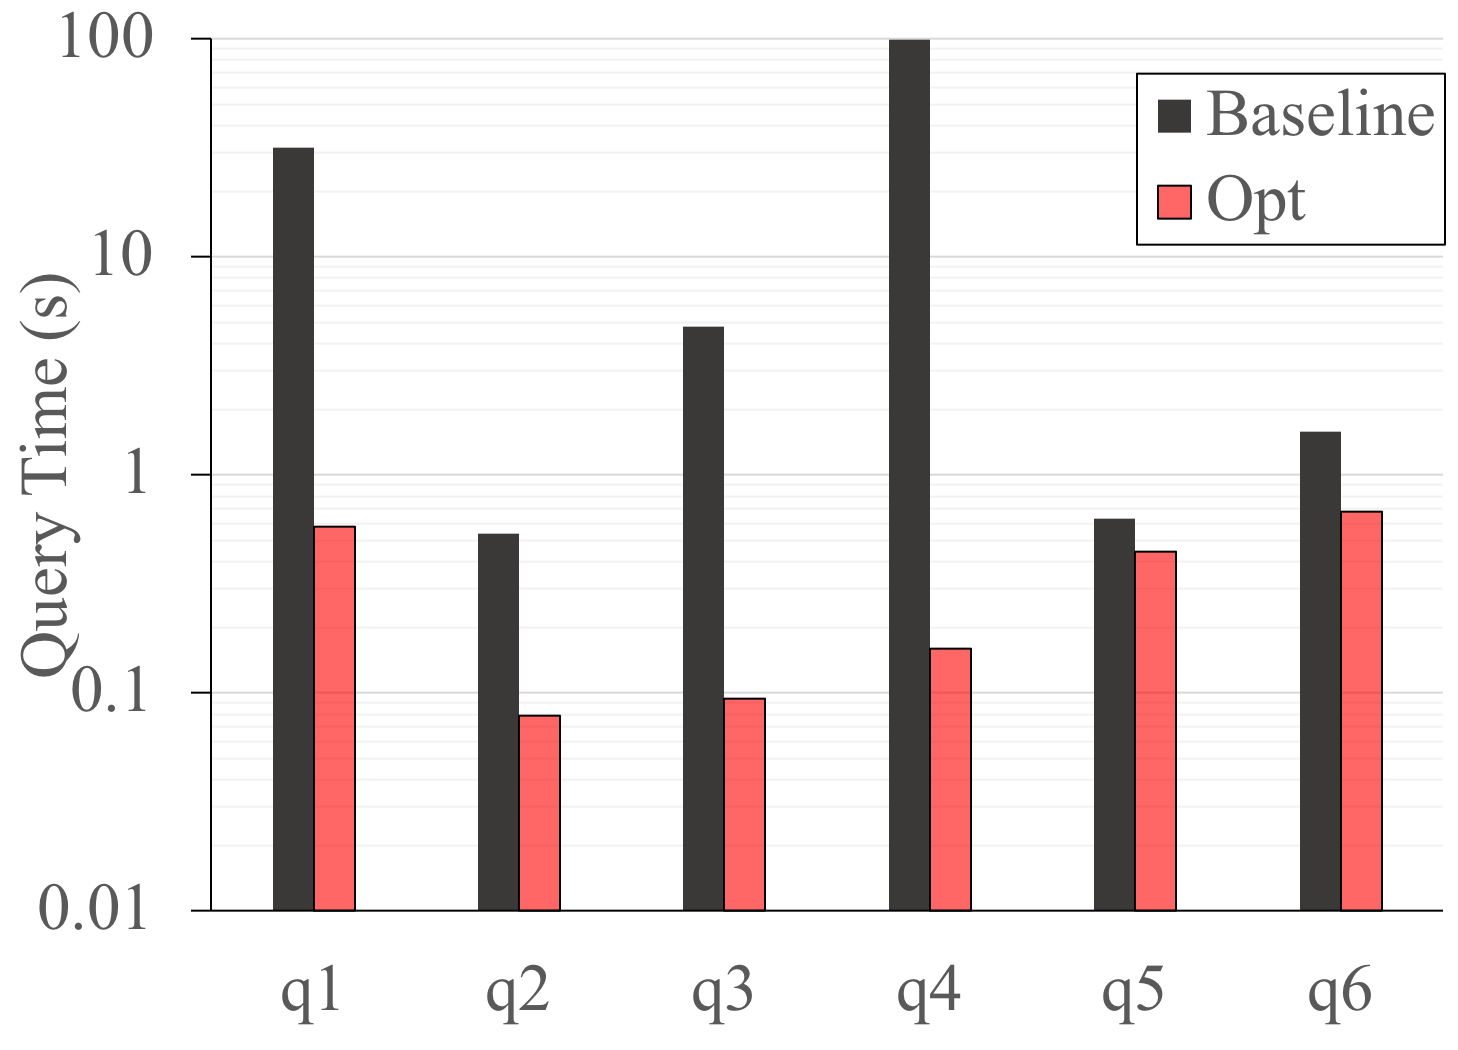
\includegraphics[width=0.7\columnwidth]{figures/query.png}
 \caption{\textsf{DeepLens} significantly speeds up ``query time'' by using indexes. The queries that match multidimensional features can be sped up by up-to 600x.  \label{query} }
\end{figure}

\subsection{The Power of Indexes}
The first question is how valuable indexes are for our benchmark dataset.
Figure \ref{query} plots the query times with and without indexing.
Our baseline is the dataflow query processing engine with no indexes.
We compare this baseline to a hand-tuned version where we manually select the best physical design for a query.

The queries that benfit the most from the indexes are ones that require image matching, up-to 612x faster for q4 and 59x faster for q1. Some queries have improvements since they leverage the lineage information and do not need to rescan the base data. q3 requires a backtracing query to match the bounding boxes and the OCR output in pixels on the original image and has a 41x improvement. Similarly, q6 runs 2.5x faster. q5 is illustrative of a query whose predicate does not benefit from any of the available indexes.

What is interesting about these improvements also illustrate the compute-bound nature of these queries.
For q1, all of the images can fit in memory.
However, the all pairs similarity comparison can be very slow.
Building a Ball-tree over one side of the join and probing with the other is a much faster approach as it reduces the number of comparisons needed.
In general, image processing algorithms are very compute intensive, so upstream operations that can reduce the number of future numerical comparisons can very significantly reduce the execution time of queries.


\begin{figure}[t]
% \vspace{-5pt}
\centering
 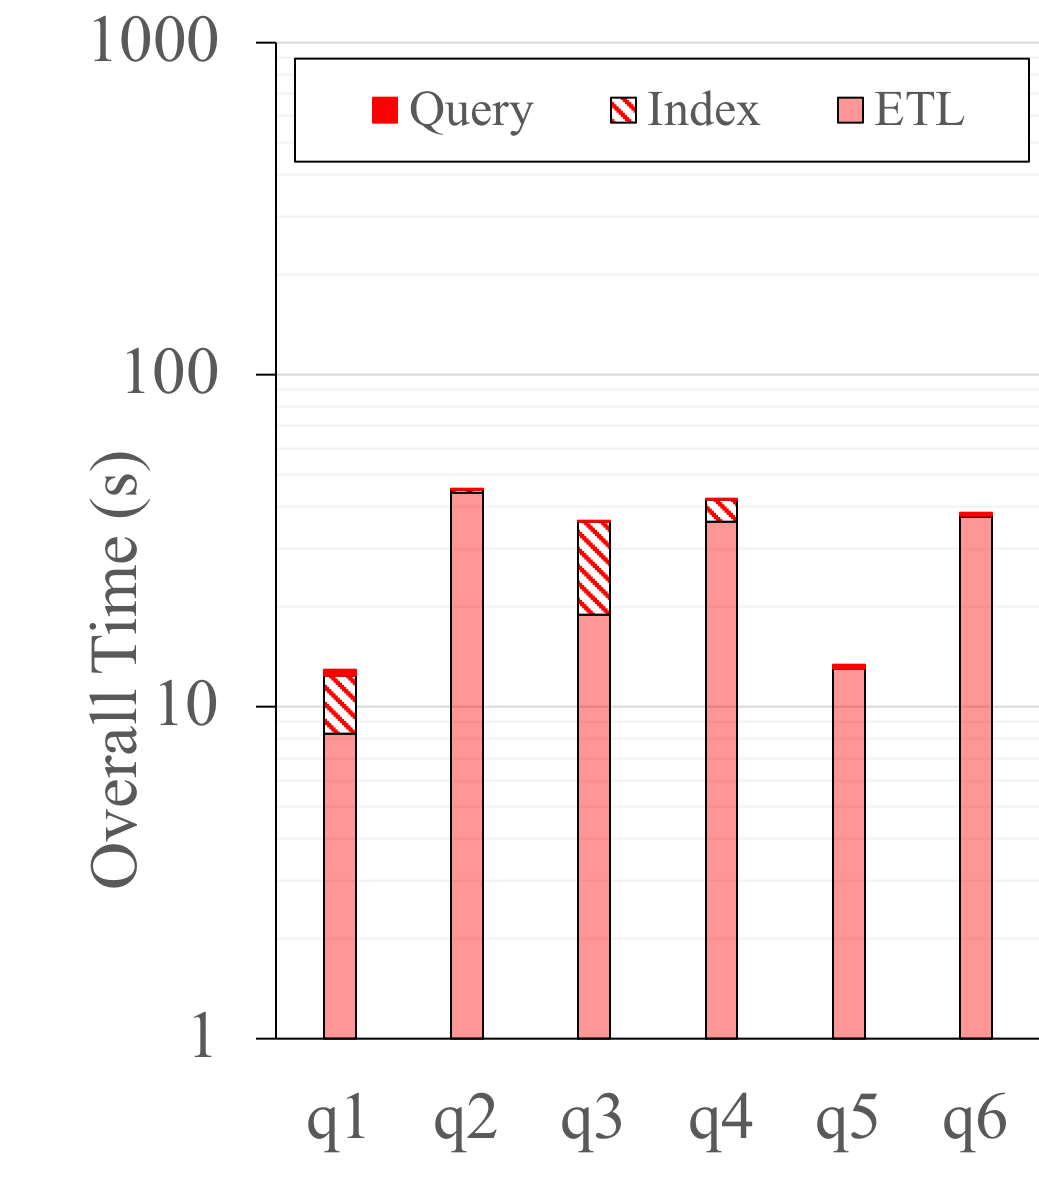
\includegraphics[width=0.46\columnwidth]{figures/indexing_b.png}
 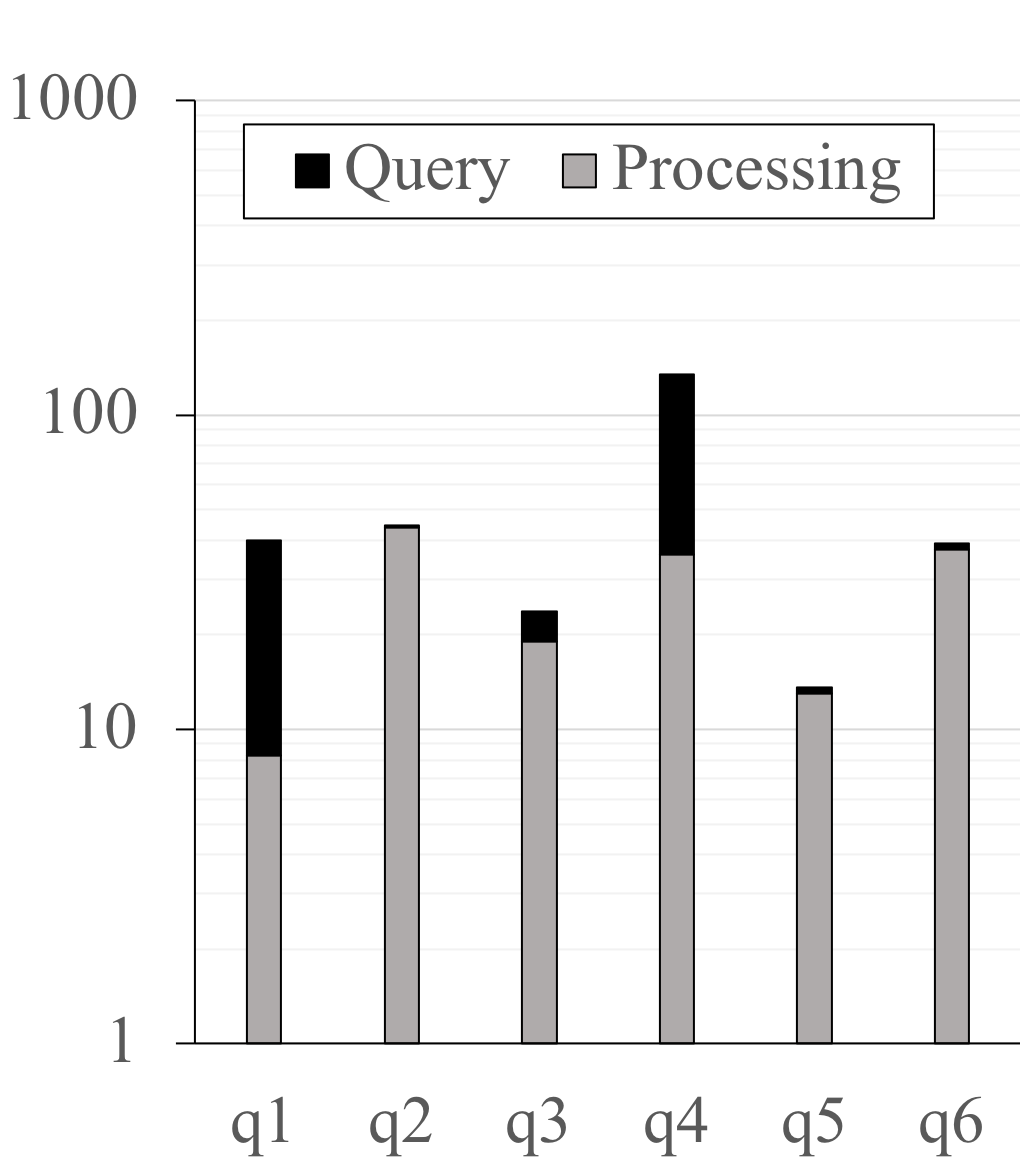
\includegraphics[width=0.49\columnwidth]{figures/indexing_a.png}
 \caption{We evaluate the pipeline runtime, including ETL and index creation, for an optimized \textsf{DeepLens} (red) vs. the baseline (black). On many queries it is beneficial to materialize intermediate results and build indexes to speed up future performance. Indexing has a relatively small overhead given the compute-intensive nature of the queries. \red{We could change Processing to ETL and show the 3 steps in each column in this order: ETL + Index creation + Query execution.} \label{index} }
\end{figure}

\begin{figure}[t]
% \vspace{-5pt}
\centering
 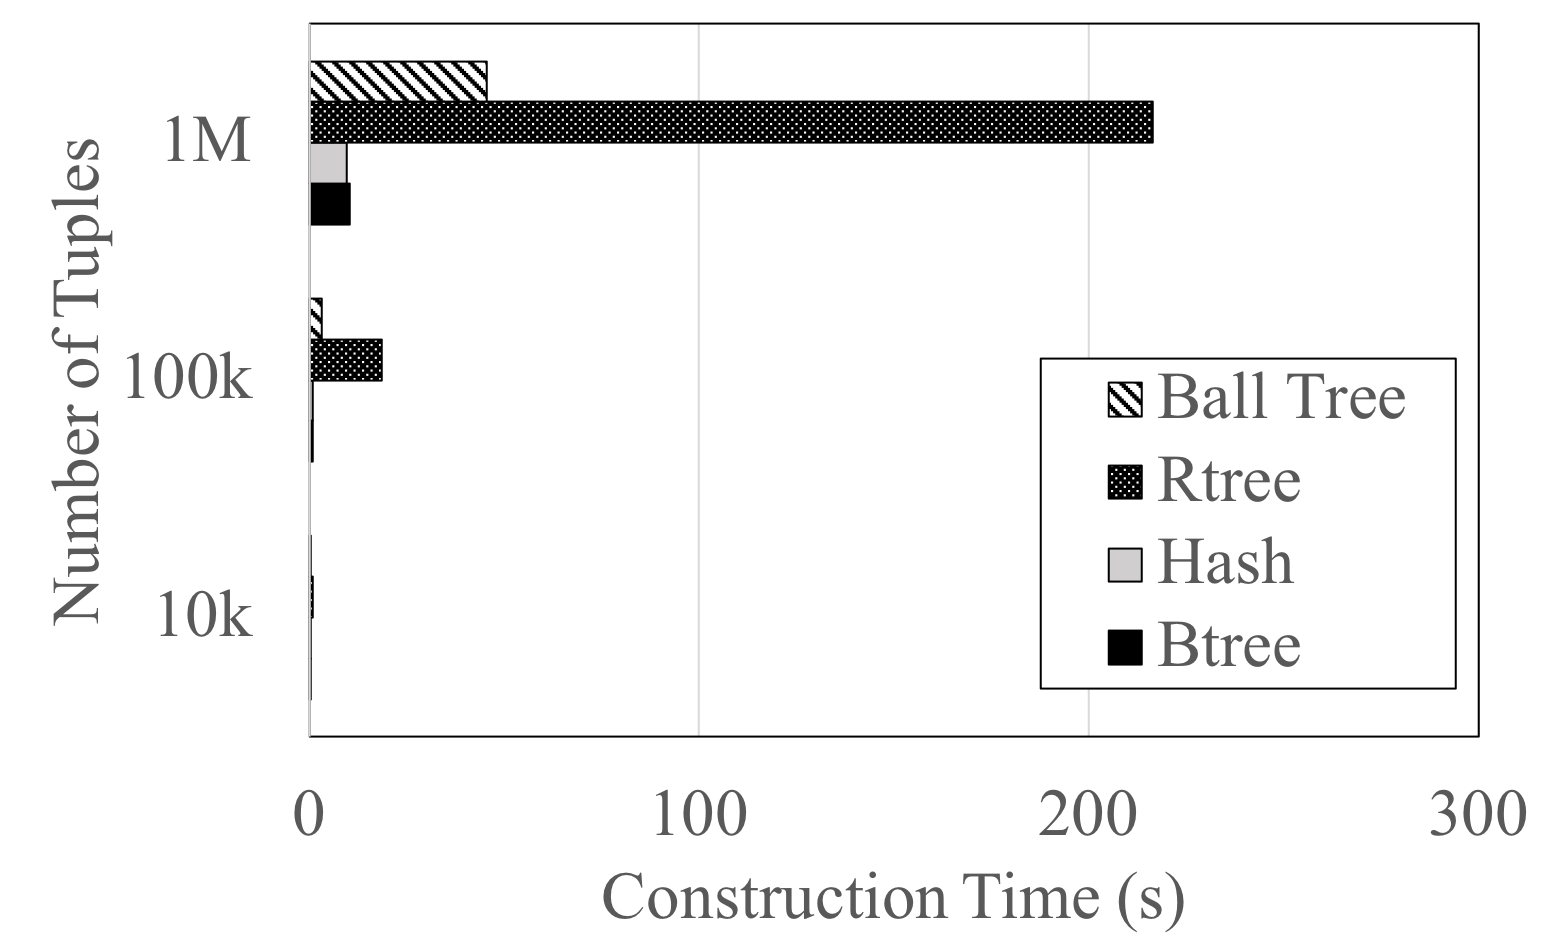
\includegraphics[width=0.8\columnwidth]{figures/indexing.png}
 \caption{Building multidimensional indexes can be very costly and initial experiments indicate that construction time scales poorly with data. \label{indexbuild} }
\end{figure}

\subsection{Overhead For Indexing}
One might think that persisting an index incurs a large overhad; however, it is small relative to the compute cost of the entire pipeline including the ETL.
Even disregarding the fact that indexes can be reused by other queries and their cost amortizes, several of the queries execute faster even if the indexes are built ``on-the-fly'' (Figure \ref{index}).
For example, q1 executes nearly 5 times faster than the baseline and q4 executes 3.5 times faster than the baseline.
As with the previous results, this is largely due to the compute-intensive nature of those queries.
The index significantly reduces the number of image matching operations which dominate the runtime, and thus, the cost of building and persisting the index is offset.

The indexes with largest overhead to build are the spatial indexes.
Figure \ref{indexbuild} plots the construction time of the multidimensional and single dimensional indexes supported in \textsf{DeepLens} as a function of the number of tuples indexed.
The R-Tree is nearly 20x slower to construct than a B+ Tree.
However, there are some mitigating factors that are interesting to consider in future work.
Since visual analytics is approximate by nature, perhaps exact multidimensional indexing is unnecessary. 
For some workloads may suffice to apply single dimensional indices and merge results with independence assumptions.
For others, locality sensitive hashing or similar approximations may suffice.

\begin{figure}[t]
% \vspace{-5pt}
\centering
 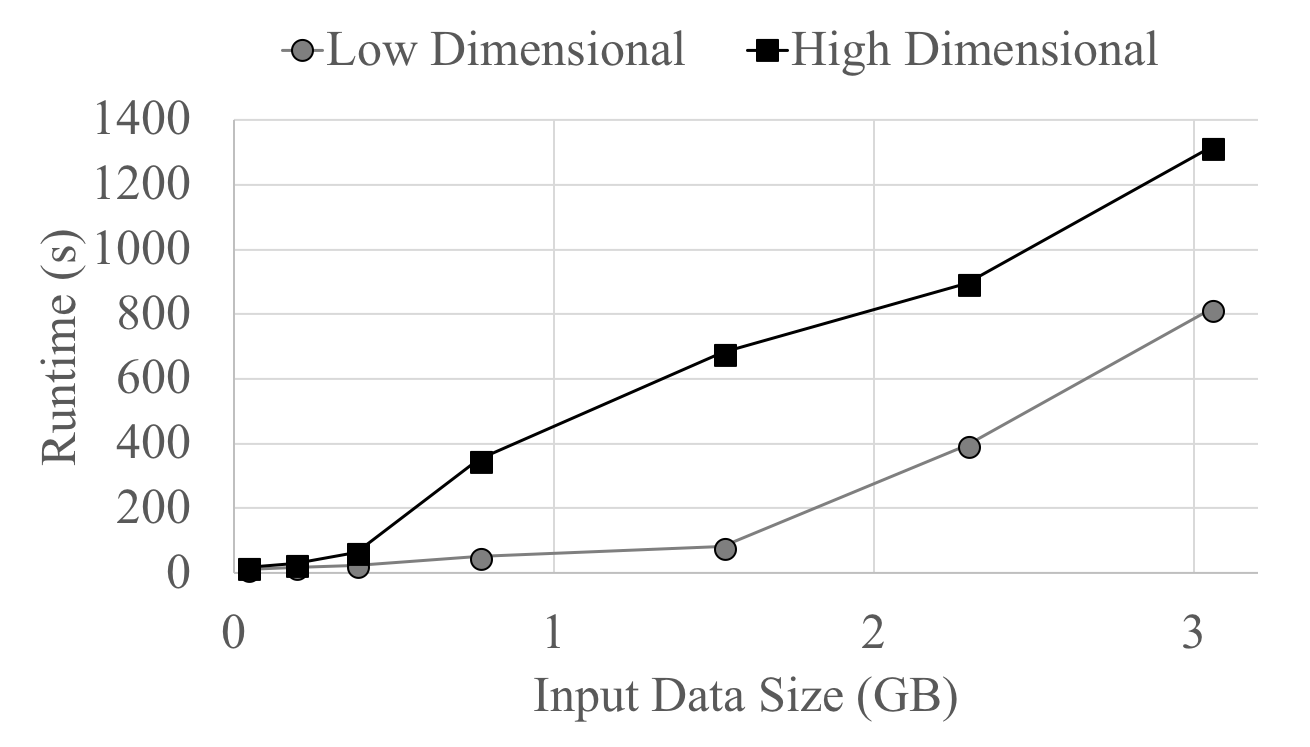
\includegraphics[width=\columnwidth]{figures/spatialjoin.png}
 \caption{We evaluate the execution time of a Ball-Tree join as function of the size of the indexed relation in the high-dimensional and low-dimensional case. As the data structure is increasingly filled the execution time grows non-linearly. \red{Probably we could change the label on the x axis to Number of Tuples to match the y axis in Figure 4.} \label{join} }
\end{figure}


\subsection{Cost-Based Optimization}
To avoid a large library of hand-written rules, the natural question to ask is whether it is possible to build a cost-based query optimizer for this system.
In cost-based query optimization, the optimizer uses a cost model to evaluate the cost of different query execution plans. We find that operators in \textsf{DeepLens} pose a few challenges for cost-based optimization. 

Figure \ref{join} illustrates the difficulties with the execution time of a Ball-Tree join as function of the size of the indexed relation in the high-dimensional and low-dimensional case. As the data structure is increasingly filled the execution time grows non-linearly. The non-linearity is also data-dependent and is more extreme in higher dimensional data. Accurately modeling the relationship between input relation size and operator cost is crucical for cost-based query optimization. Non-linearities are also known to affect standard join ordering heuristics.

\begin{figure}[t]
% \vspace{-5pt}
\centering
 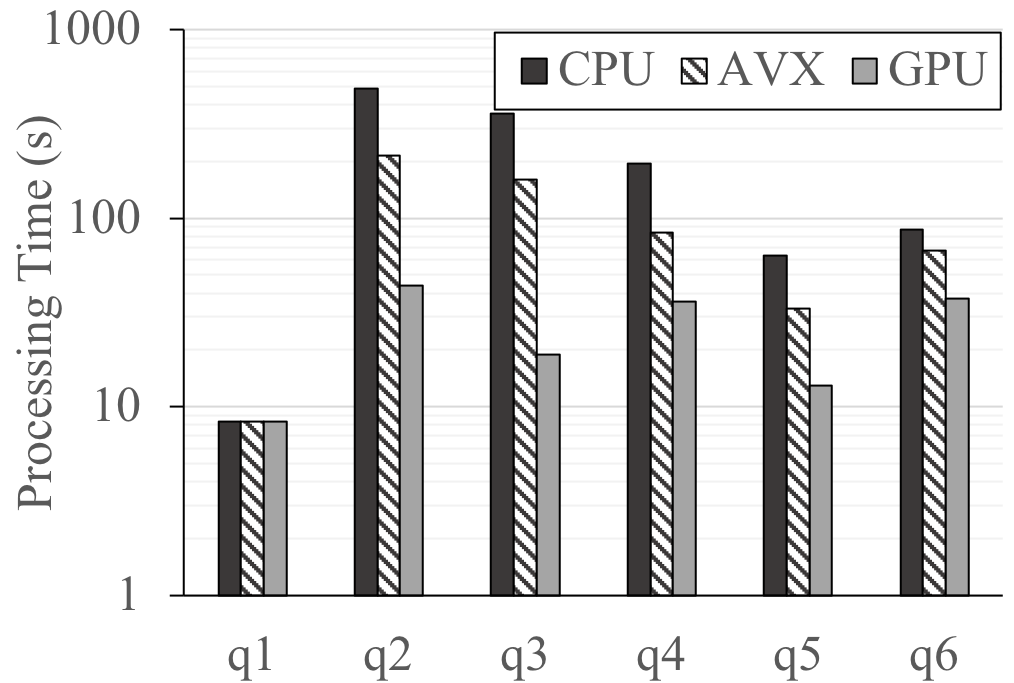
\includegraphics[width=0.8\columnwidth]{figures/build.png}
 \caption{The execution architecture has a considerable impact on the processing time.  \label{build} }
\end{figure}

Compute-bound operations are also, by nature, sensitive to the underlying system architecture and execution engine. Figure \ref{build} plots the processing time on each of the six benchmark queries for a vanilla CPU implementation (CPU), a vectorized neural network implementation (AVX), and a GPU implementation (GPU). Just by changing the underlying execution architecture there were up-to 12x changes in execution time. 



\section{Conclusion and Future Work}
Images and video are the frontier of modern data management.
The growing maturity of neural networks for image prediction and segmentation problems has made visual analytics an attractive and inter-discplinary field of study.
We explored the intersection of these neural network models and data management by designing a query processing engine called \textsf{DeepLens}.

\textbf{TODO}

%\input{acks.tex}




%\bibliographystyle{abbrv}

{
%\fontsize{8.6pt}{9.5pt} \selectfont
\bibliographystyle{abbrv}
\bibliography{ref} 
}


%\input{appendix.tex}

\end{document}
